\chapter{Introduction}
In today’s world, cardiovascular diseases (CVDs) are one of the leading causes of mortality, claiming millions of lives every year. Early detection and timely monitoring of heart health are crucial for managing these conditions effectively. However, in many rural and remote areas, access to advanced healthcare facilities is limited, leaving a significant portion of the population at risk of undiagnosed heart conditions. 

Imagine a scenario: A middle-aged farmer working in a rural area experiences occasional chest discomfort but dismisses it due to lack of access to medical facilities. One day, he suffers a major heart event because his condition went undetected for years. This is not just an isolated case but a recurring reality in underserved regions. What if there was a device that could have detected his heart condition earlier, allowing timely intervention?  

Electrocardiography (ECG) is an indispensable tool for diagnosing cardiac conditions by analyzing the heart's electrical activity. However, conventional ECG systems—often multi-lead, hospital-grade machines—pose barriers in rural and low-resource settings due to high costs, bulkiness, and the requirement for trained personnel.

Our project - \textbf{Micro-ECG} aims to eliminate these limitations by offering a fully portable, battery-powered, single-lead ECG system that uses:
\begin{itemize}
    \item A WiFi-based microcontroller (ESP8266) for communication.
    \item A real-time, browser-based user interface via captive portal.
    \item Hardware-level noise suppression using op-amps and RC filters.
    \item Frontend ECG signal filtering using hand-crafted JavaScript code.
\end{itemize}

Unlike Bluetooth-based systems or mobile apps, Micro-ECG works independently across devices, requiring only a browser to operate. With both on-device and external chest electrodes, it captures and visualizes cardiac signals accurately.






\chapter{Background}
The heart generates electrical impulses via the sinoatrial (SA) node, which propagate through the atria, AV node, and ventricles. This electrical conduction results in waveform patterns—P wave, QRS complex, and T wave—which an ECG captures.

\begin{figure}[H]
    \centering
    \includegraphics[width=0.7\textwidth]{images/electrical_heart.jpg}
    \caption{The electrical conduction system of the heart}
    \label{fig:electrical_heart}
\end{figure}

\begin{figure}[H]
    \centering
    \includegraphics[width=0.7\textwidth]{images/pqrst.jpg}
    \caption{Normal ECG signal pattern with signal points}
    \label{fig:pqrst}
\end{figure}

Traditional 12-lead ECG machines provide comprehensive cardiac information but:
\begin{itemize}
    \item Are expensive (INR 20,000+).
    \item Require hospital-grade calibration.
    \item Depend on skilled interpretation.
\end{itemize}

\begin{figure}[H]
    \centering
    \includegraphics[width=0.7\textwidth]{images/hospital_ecg.jpg}
    \caption{Traditional Hospital ECG Machine}
    \label{fig:hospital_ecg}
\end{figure}

For early detection, especially of rhythm abnormalities like bradycardia or tachycardia, a single-lead solution is sufficient. This makes the single-lead ECG valuable for first-line screening, community health workers, and telemedicine.







\chapter{System Architecture}

\section{Block-Level Architecture}
The device consists of the following major subsystems:
\begin{enumerate}
    \item \textbf{Electrode Interface:} Captures surface potential using LA/RA finger contacts or optional chest leads.
    \item \textbf{Analog Front-End:} Uses AD8232 IC with discrete RC filter stages to suppress motion noise and 50Hz interference.
    \item \textbf{Microcontroller Unit:} ESP8266 with 10-bit ADC, serving both the UI and WebSocket data stream.
    \item \textbf{UI System:} Hosted from internal flash, drawn on HTML5 canvas, processes incoming ADC samples.
    \item \textbf{Battery and Power Management:} A 1200mAh Li-ion battery powers all modules with a Micro-USB port limited to charging and flashing.
\end{enumerate}

\begin{figure}[H]
    \centering
    \includegraphics[width=0.8\textwidth]{images/ecg_block_diagram.jpg}
    \caption{ECG block diagram}
    \label{fig:ecg_block_diagram}
\end{figure}

\section{Data Flow Overview}
The ECG signal path is as follows:
\begin{itemize}
    \item \textbf{Step 1:} Electrical signal picked up via skin contact.
    \item \textbf{Step 2:} Passed to AD8232, which filters, amplifies, and outputs analog ECG signal.
    \item \textbf{Step 3:} ESP8266 samples the analog ECG at 200–500Hz.
    \item \textbf{Step 4:} Packets of ADC values are streamed via WebSocket.
    \item \textbf{Step 5:} HTML+JS frontend buffers and renders the waveform in real time.
\end{itemize}

\begin{figure}[H]
    \centering
    \includegraphics[width=0.7\textwidth]{images/dso_block_diagram.jpg}
    \caption{Analog to Digital Signal flow  block diagram}
    \label{fig:dso_block_diagram}
\end{figure}

\section{Key Features}
\begin{itemize}
    \item Real-time visualization via any browser without app installation.
    \item WebSocket-based data delivery ensures low latency.
    \item Captive portal works even without internet.
    \item Chest lead option increases signal fidelity.
    \item Lightweight filtering on hardware and software layers.
\end{itemize}






\chapter{Hardware Design}

\begin{figure}[H]
    \centering
    \includegraphics[width=0.7\textwidth]{images/proto_overview.png}
    \caption{Prototype Overview}
    \label{fig:proto_overview}
\end{figure}
{\small
\begin{enumerate}
    \item \textbf{LA \& RA Electrodes (Touch Type):} Finger placement electrodes for Left Arm (LA) and Right Arm (RA) detection. These are the primary contact points for quick ECG readings.
    \item \textbf{Heart LED Indicator:} Blinks in sync with the detected heart rhythm. Also shows device power status.
    \item \textbf{Charging Status LED:} \\ \textcolor{red}{Red} – Charging,\\ \textcolor{blue}{Blue} – Fully charged.
    \item \textbf{External Electrode Port:} Alternative electrode input, typically for chest placement using gel electrodes for improved accuracy.
    \item \textbf{Slide Switch (Charge-Off-On):} \\ \textit{Charge} – Enables charging without powering on the device.\\ \textit{Off} – Completely powered off.\\ \textit{On} – Powers the device for use.
    \item \textbf{Micro-USB Port:} Used for charging and firmware updates only. \\ \textbf{Note:} Do not use the device while charging to avoid inaccurate results.
\end{enumerate}
}
\section{Electrodes}
Micro-ECG provides two types of electrode input:
\begin{itemize}
    \item \textbf{Integrated Electrodes (Top):} LA and RA contacts on the top surface for direct finger placement. Fingerpads are made of copper wire, ensuring good skin contact. Wider surface contact improves signal quality.
    \item \textbf{External Chest Electrode Port:} A front-facing 3.5mm port allows optional chest-mounted electrode placement. This method provides higher signal amplitude and better baseline stability due to reduced motion artifacts.
\end{itemize}

\section{Analog Front-End Circuitry}
At the core is the \textbf{AD8232} AFE (Analog Front-End), chosen for its compact ECG functionality. The IC includes:
\begin{itemize}
    \item Instrumentation amplifier with high CMRR.
    \item Adjustable gain using external resistor ($G = 1 + \frac{100k\Omega}{R_G}$).
    \begin{figure}[H]
    \centering
        \includegraphics[width=0.7\textwidth]{images/bio_Ins.jpg}
        \caption{BioInstrumentation Amplifier topology}
        \label{fig:bioIns_block}
    \end{figure}
    \item Internal high-pass (0.5 Hz) and low-pass (~40 Hz) filters for motion and line noise rejection.
\end{itemize}

\section{AMPLIFIER}
We use the AD8232\cite{AD8232} bioinstrumentation amplifier, a reliable choice for portable ECG devices. This amplifier is designed to capture the heart’s weak electrical signals and amplify them for accurate processing. It offers high precision, low power consumption, and effective signal enhancement, making it suitable for mobile applications where battery efficiency and signal clarity are crucial.
\begin{figure}[H]
    \centering
    \includegraphics[width=0.7\textwidth]{images/ad8232_block.jpg}
    \caption{AD8232 block diagram\cite{AD8232}}
    \label{fig:AD8232_block}
\end{figure}

\textbf{Additional Filtering:}
\begin{itemize}
    \item \textbf{RC low-pass filter:} After AD8232 output, an RC filter (typically 1kΩ + 10$\mu$F) suppresses 50/60Hz hum.
    \item \textbf{Decoupling capacitors:} Used near the supply rails for stability.
\end{itemize}

\begin{figure}[H]
    \centering
    \includegraphics[width=0.6\textwidth]{images/ad8232_circuit.jpg}
    \caption{AD8232 circuit diagram\cite{AD8232}}
    \label{fig:AD8232_circuit}
\end{figure}

\section{Power Supply}
\begin{itemize}
    \item \textbf{Battery:} 1200mAh Li-ion, securely fixed inside the enclosure.
    \item \textbf{Charging Circuit:} TP4056-based charger IC with overcurrent protection.
    \item \textbf{Voltage Regulation:} External LDO of RT9080 - 3.3v used; draws ~120mA peak with WiFi.
\end{itemize}

\section{Enclosure and Controls}
\begin{itemize}
    \item \textbf{Heart Symbol LED:} Located at top-center, pulses with heart rhythm and indicates power.
    \item \textbf{Charge-Off-On switch:} Controls power flow.
    \item \textbf{Red LED:} Glows during charging.
    \item \textbf{Blue LED:} Indicates full charge.
\end{itemize}






\chapter{Signal Acquisition and Filtering}

\section{Signal Characteristics}
Typical ECG voltages are 0.5–3 mV, requiring careful amplification. The AD8232 amplifies these small signals to ~1V peak-to-peak for easy sampling by the 10-bit ADC of the ESP8266.

\section{ADC Considerations}
\begin{itemize}
    \item ESP8266 ADC reads 0–1V with 10-bit resolution.
    \item An external voltage divider biases the analog input to ~0.5V baseline (AC-coupled).
    \item The effective resolution is $\frac{1V}{1024} \approx 0.976mV$ per ADC step.
\end{itemize}

\section{Filtering Pipeline}
\textbf{Hardware Filtering:}
\begin{itemize}
    \item High-pass (0.5 Hz) to eliminate baseline wander (from respiration).
    \item Low-pass (~40 Hz) to remove muscle noise.
\end{itemize}

\textbf{Frontend JS Filtering:}
\begin{itemize}
    \item Rolling average (N = 5 to 10 samples).
    % \item Optional digital IIR high-pass to stabilize drift.
\end{itemize}

\section{Noise Sources Addressed}
\begin{itemize}
    \item \textbf{Power Line Noise:} Minimized by RC filter + good PCB routing.
    \item \textbf{Motion Artifact:} Reduced via chest electrodes and tight contact.
    % \item \textbf{EMI:} Shielded wiring and star grounding reduce interference.
\end{itemize}






\chapter{Software Architecture}

\section{ESP8266 Firmware Design}
Firmware is written using the Arduino core for ESP8266. Major modules include:
\begin{itemize}
    \item \textbf{WiFi Access Point:} Default SSID “Micro\_ECG\_RANMPGroupF”, no password.
    \item \textbf{Captive Portal:} Uses DNS hijack and local HTTP server.
    \item \textbf{WebSocket Server:} For real-time ADC streaming.
    \item \textbf{ADC Sampling:} Samples analog ECG at ~250Hz using a timer interrupt.
    \item \textbf{Frame Batching:} Sends 70-80 samples per WebSocket frame for efficiency.
\end{itemize}

\begin{figure}[H]
\centering
\includegraphics[width=0.6\textwidth]{images/firmware-diagram(8266).png}
\caption{ESP8266 Firmware Architecture}
\label{fig:firm8266_diagram}
\end{figure}


\section{Sampling Optimization}
\begin{itemize}
    \item ADC read in ISR (Interrupt Service Routine) using \texttt{timer1}.
    \item Samples placed into ring buffer.
    \item Main loop dispatches WebSocket events and serves UI files.
\end{itemize}

\section{OTA and Updates}
Firmware updates are performed via USB using Espressif Flash Download Tools [see official documentation from https://www.espressif.com/en ].






\chapter{Frontend Web User Interface}

\section{Architecture Overview}
The frontend is written in plain HTML5, CSS, and JavaScript, hosted locally from ESP8266 flash. No backend or internet is required. The user connects to the device via WiFi, and the interface is served directly.

\begin{figure}[H]
\centering
\includegraphics[width=0.6\textwidth]{images/firmware-diagram(frontend).png}
\caption{Frontend Firmware Architecture}
\label{fig:firm_frontend_diagram}
\end{figure}

\section{Canvas Rendering Engine}
The ECG signal is plotted on an HTML5 `<canvas>` element. Core design:
\begin{itemize}
    \item \textbf{Canvas Width:} Responsive; typically 300–1200px or more depending on device screen.
    % \item \textbf{Y-Scale Calculation:} Autoscaled to keep peak-to-peak signal visible.
    \item \textbf{X-Axis Mapping:} Buffer size determines how many samples fit on screen.
    % \item \textbf{Grid Lines:} Vertical (time divisions), Horizontal (amplitude markers).
\end{itemize}

\section{Signal Buffer Handling}
\begin{itemize}
    \item Uses a JavaScript array (`data\_buffer[]`) to hold recent ADC values.
    \item Buffer size is set to match screen width (e.g., 1000 samples = 5s window at 200Hz).
    \item Incoming WebSocket samples are pushed, old values popped.
    \item Dynamic range detection adjusts gain (volts/div) and vertical centering.
\end{itemize}

\section{Filtering and Scaling}
\begin{itemize}
    \item Basic smoothing via moving average (optional toggle).
    \item JavaScript-based digital high-pass for baseline correction.
    % \item Y-axis scale auto-adjusts to match incoming waveform amplitude.
\end{itemize}

\section{Event Handling}
\begin{itemize}
    \item \textbf{Resize Event:} Rescales canvas and resets buffer.
    % \item \textbf{Touch Support:} Can add tap-to-freeze or mark timestamps.
    \item \textbf{Error Events:} Notifies disconnection, reconnection, or invalid data.
\end{itemize}

\section{AI Integration}
\begin{itemize}
    \item The frontend can connect to a third-party ECG AI API.
    \item Sample batch is sent as JSON POST.
    \item Resulting classification (e.g., normal/AFib) is shown below the canvas in AI tab.
    \item Used for advanced diagnostics, requires internet access.
\end{itemize}






\chapter{User Operation Guide}

\section{Getting Started}
\subsection{Power On}
Slide \textbf{POWER} switch to ON. The heart LED should start blinking.
(If it doesn't blink, ensure the device is charged.)
\subsection{Connect to Wi-Fi}
On your mobile or computer, connect to the device’s Wi-Fi hotspot.
(Note: Only supports 2.4GHz networks.)
\subsection{Open the User Interface}
Once connected to the ECG device's Wi-Fi, a screen should automatically pop up with the web interface. \\
If it doesn’t open by itself, just open any browser (Chrome recommended) and go to: \\
http://172.217.28.1 \\
Chrome tested on mobile, desktop, and laptop — works on cross-platform.
\subsection{ECG Display}
The graph canvas may initially show random noise if electrodes are open.

\subsection{Electrodes}
\begin{itemize}[leftmargin=*]
  \item \textbf{Finger:} Touch LA \& RA on top of the device. OR,
  \item \textbf{Chest:} Connect external electrode (Front-Left side)
\end{itemize}

\subsection{Take Reading}
Once the waveform is stable , no noise on the screen, hold still and observe the heart rate.

\section{Parameters}
\begin{figure}[H]
    \centering
    \includegraphics[width=0.7\textwidth]{images/ss/view-param.png}
    \caption{User interface Parameters view}
    \label{fig:ss_param_view}
\end{figure}
\begin{itemize}[leftmargin=*]
    \item \textbf{Heart Rate (BPM):} -  Beats per minute calculated in real-time.
    \item \textbf{QRS Duration:} -  Time interval of the QRS complex, indicating ventricular depolarization.
    \item \textbf{QT Interval:} -  Total time for ventricular depolarization and repolarization.
    \item \textbf{PR Interval:} -  Time from the start of the P wave to the start of the QRS complex.
    \item \textbf{ST Interval:} -  Segment between the end of the S wave and the beginning of the T wave.
\end{itemize}

\section{AI Assistant}
\begin{figure}[H]
    \centering
    \includegraphics[width=0.7\textwidth]{images/ss/view-ai.png}
    \caption{User interface AI view}
    \label{fig:ss_ai_view}
\end{figure}
\begin{itemize}[leftmargin=*]
    \item \textbf{Function:} -  ECG data send to a third-party AI for anomaly detection.
    \item \textbf{How to Use:} -  Click on the "Get Assistance" button to initiate the AI analysis.
\end{itemize}

\section{Controls}
\begin{figure}[H]
    \centering
    \includegraphics[width=0.7\textwidth]{images/ss/view-controls.png}
    \caption{User interface Controls view}
    \label{fig:ss_controls_view}
\end{figure}
\begin{itemize}[leftmargin=*]
    \item \textbf{HOLD:} -  Pauses the real-time ECG display.​
    \item \textbf{RECORD:} -  Starts recording the ECG data.​
    \item \textbf{CLEAR:} -  Clears the current ECG graph from the display.​
    \item \textbf{SNAP:} -  Captures a snapshot of the current ECG graph.​
    \item \textbf{TIME/DIV (-/+):} -  Adjusts the time scale of the ECG graph.​
    \item \textbf{VOLT/DIV (-/+):} -  Adjusts the voltage scale of the ECG graph.
    \item \textbf{POSITION VERTICAL (\ding{115}/\ding{116}):} -  Moves the ECG graph up or down.​
    \item \textbf{POSITION HORIZONTAL (\prevtrack/\nexttrack):} -  Moves the ECG graph left or right.​
\end{itemize}

\section{Recordings}
\begin{figure}[H]
    \centering
    \includegraphics[width=0.7\textwidth]{images/ss/view-record.png}
    \caption{User interface Recordings view}
    \label{fig:ss_record_view}
\end{figure}
\begin{itemize}[leftmargin=*]
    \item \textbf{IMPORT (.json):} -  Allows importing of ECG data in JSON format.
    
    \item \textbf{Accessing Recordings:} -  Recorded ECG sessions are listed with timestamps in the RECORDINGS section..​
    \item \textbf{Downloading Recordings:} -  Click on the download (\downleftarrow) icon next to a recording to download the data..​
    \item \textbf{Deleting Recordings:} -  Click on the ($\times$) icon next to a recording to delete it.
\end{itemize}

\section{Settings (Not available - Planned)}
% \begin{itemize}[leftmargin=*]
%   \item WiFi SSID change
%   \item Adjust SPS
%   \item Factory Reset
%   \item Firmware update access
% \end{itemize}

\section{Troubleshooting}
\begin{itemize}
    \item \textbf{No Heart LED Blinking:} \\
    Ensure the device is charged. Slide the power switch OFF and ON again.

    \item \textbf{Cannot Connect to Wi-Fi:} \\
    Confirm your device supports 2.4GHz Wi-Fi. Restart the ECG device and try again.

    \item \textbf{Web Interface Doesn’t Open Automatically:} \\
    Check sign-in notification | open a browser manually (Chrome recommended) and enter\\ \texttt{http://172.217.28.1}.

    \item \textbf{Weak signal:} \\
    Possible Cause: Dry skin, poor contact | Moisten fingers slightly or use external electrode.

    \item \textbf{Data delay in UI:} \\
    Improve WiFi signal, Move closer to the device.

    \item \textbf{ECG Graph Shows Noise:} \\
    Ensure stable positioning, avoid movement. \\
    Make sure the electrodes are placed correctly. Wait a few seconds for the signal to stabilize. \\
    For finger electrodes, gently rub and clean the metal surface before use to improve contact. \\
    \textbf{Do not} try to rub or clean the disposable adhesive external electrodes, as this may damage them.
\end{itemize}

\section{Safety \& Maintenance}
\begin{itemize}[leftmargin=*]
  \item Keep electrodes clean and dry for optimal signal quality.
  \item Use BIS certified charger to charge via Micro-USB.
  \item Do not submerge in water or expose to excessive moisture.
  \item Don't drop or shake.
  \item Update firmware from authorised source only.
  \item Avoid applying excessive force on the device or electrodes.
\end{itemize}












\chapter{Implementation and Results}

\section{Prototype Construction}
The entire circuit—including the AD8232, ESP8266 module, charging system, and control switch—was soldered with Enameled Copper Wire and enclosed in a non-conductive plastic case. Design priorities:
\begin{itemize}
    \item Minimal footprint (pocket-sized, ~13cm x 4cm x 4cm).
    \item Direct finger placement for LA/RA.
    \item Access to external chest port.
    \item Long battery life with charging.
\end{itemize}

\begin{figure}[h]
    \centering
    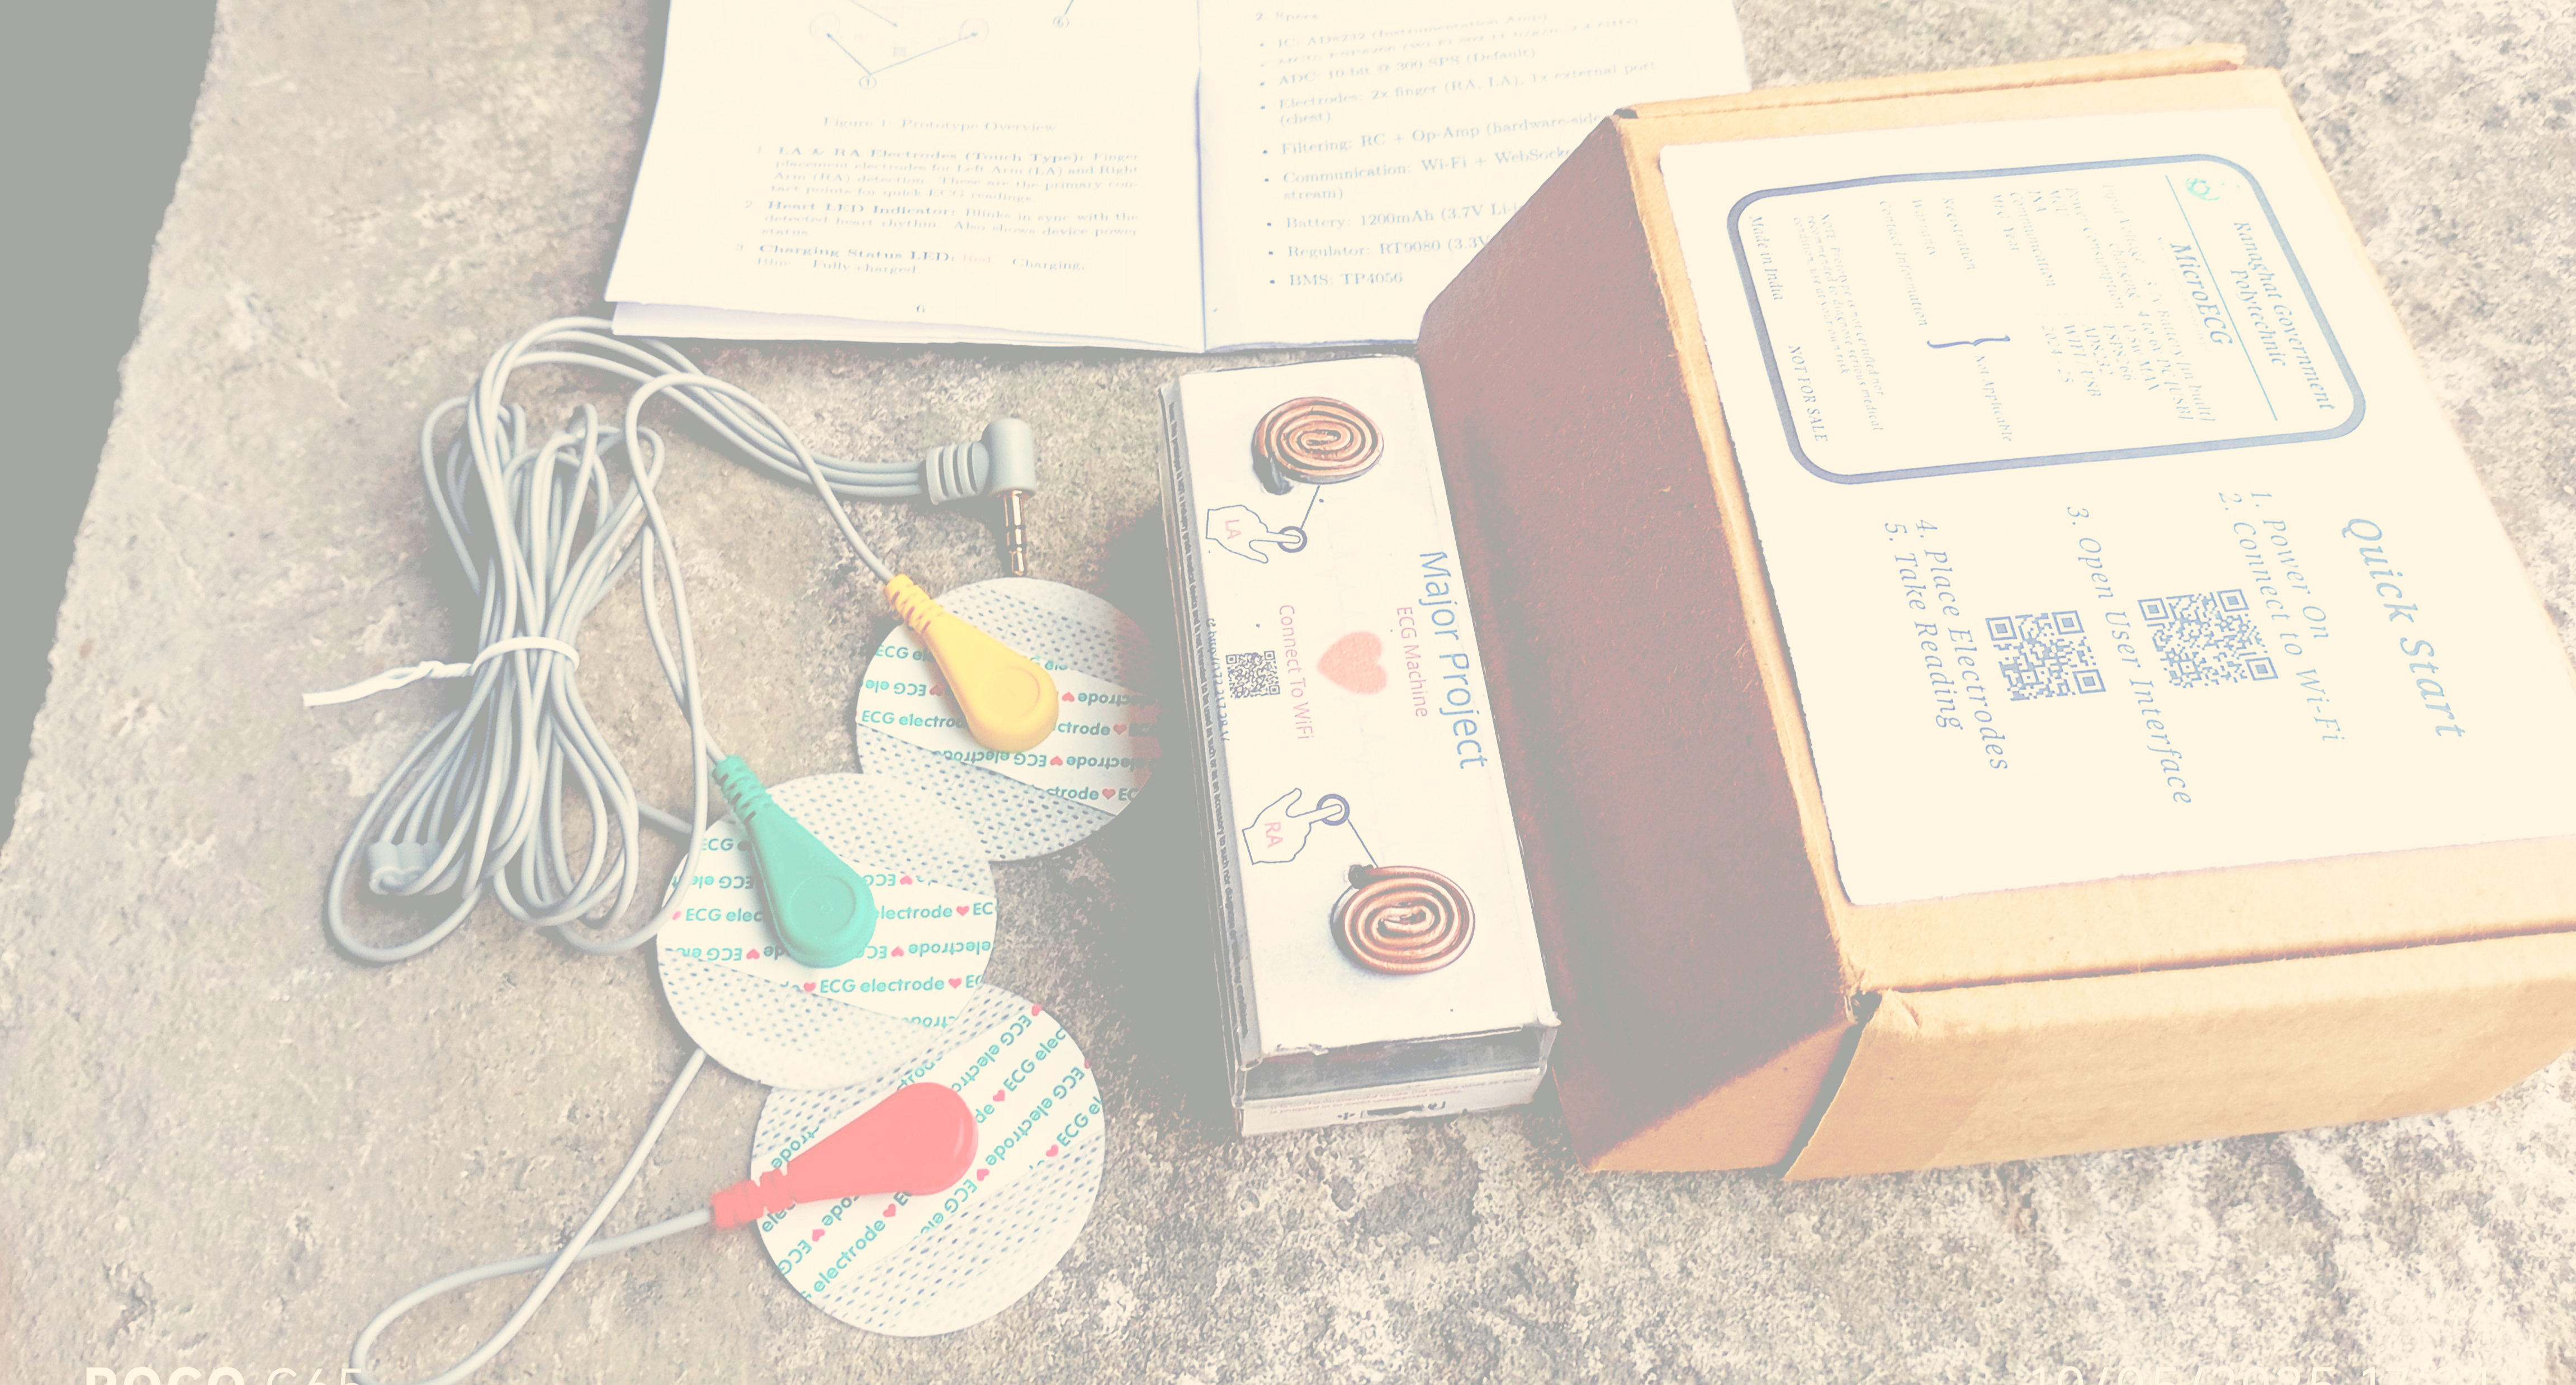
\includegraphics[width=0.75\textwidth]{images/proto.jpg}
    \caption{Final device prototype}
\end{figure}

% \section{PCB Layout Overview}
% The PCB includes separate analog and digital ground planes to minimize interference. Analog paths are shielded and routed first. The ESP8266 is mounted centrally to reduce trace length for ADC signal.

\section{Signal Stability and Noise Test}
Tests were conducted using both finger and chest electrodes. Observations:
\begin{itemize}
    \item With proper finger placement, the R-peaks are clearly visible.
    \item Chest lead usage significantly reduced baseline drift.
    \item Minor noise was handled via JavaScript-based smoothing.
\end{itemize}

\section{Web Interface Performance}
\begin{itemize}
    \item Tested on Android, iOS, Windows, and Linux.
    \item Average frame rate: ~15 fps(matches base device screen fps) with 200Hz data.
    \item Latency between ADC read and graph render: <500ms.
    \item No buffering issues observed during continuous 30-minute sessions.
\end{itemize}

\begin{figure}[h]
    \centering
    \begin{subfigure}[b]{0.45\textwidth}
        \includegraphics[width=\textwidth]{images/result-portrait.png}
        \caption{ECG signal rendering on browser from 6 different leads}
    \end{subfigure}
    \hfill
    \begin{subfigure}[b]{0.45\textwidth}
        \includegraphics[width=\textwidth]{images/result-params.png}
        \caption{ECG signal parameters automatic algorithmic analysis}
    \end{subfigure}
    \caption{ECG signal and parameters - RESULT}
\end{figure}
\begin{figure}
    \centering
    \begin{subfigure}[b]{0.45\textwidth}
        \includegraphics[width=\textwidth]{images/result-AI.png}
        \caption{ECG signal AI Analysis from third-party AI agent API endpoint}
    \end{subfigure}
    \hfill
    \begin{subfigure}[b]{0.45\textwidth}
        \includegraphics[width=\textwidth]{images/result-recordings.png}
        \caption{ECG signal recording/logging and snapshot}
    \end{subfigure}
    \caption{AI, recording/logging, snapshot - RESULT}
\end{figure}
% \begin{figure}[h]
%     \centering
%     % \includegraphics[width=0.75\textwidth]{images/dso_block_diagram.jpg
%     \caption{Live ECG signal rendering on browser}
% \end{figure}






\chapter{Future Scope}

\section{Multi-Lead Expansion}
The current architecture supports one lead. A future version can include:
\begin{itemize}
    \item Switchable analog multiplexers for multiple inputs.
    \item ESP32 with multiple ADCs for parallel acquisition.
    \item Software logic for lead selection and waveform labeling.
\end{itemize}

\section{AI-Assisted Diagnostics}
Currently, AI classification is supported via external APIs. Future integration may include:
\begin{itemize}
    \item On-device TinyML inference.
    \item Real-time rhythm classification (AFib, bradycardia).
    \item Training models on locally collected ECG data.
\end{itemize}

\section{Bluetooth Compatibility}
Adding BLE for optional use with mobile apps. ESP32 supports dual-mode communication.

\section{Remote Monitoring and Logging}
With internet uplink, data can be:
\begin{itemize}
    \item Stored on cloud databases.
    \item Viewed remotely by doctors via web dashboards.
    \item Annotated and replayed for longitudinal studies.
\end{itemize}

\section{Design for Mass Deployment}
\begin{itemize}
    \item Improve enclosure durability (IP-rated).
    \item Medical-grade electrode support.
    \item Certifications for clinical trials and diagnostics.
\end{itemize}




\chapter{Conclusion}

The aim of this project was to conceptualize, design, and implement a fully functional, real-time ECG monitoring system that integrates analog and digital subsystems into a single, self-contained platform. From signal acquisition to wireless visualization, the system demonstrates a complete end-to-end solution rooted in precision sensing, signal conditioning, embedded programming, and user-interface development.

Through the integration of bio-signal amplification, hardware noise filtering, ADC-based data acquisition, and WiFi-enabled microcontroller interfacing, the project showcases how complex physiological signals can be processed and presented in a low-latency digital form without relying on external computing infrastructure.

Key outcomes include:
\begin{itemize}
    \item A self-powered, embedded system for biomedical signal monitoring.
    \item Custom hardware design supporting both finger and chest electrode inputs.
    \item Real-time, browser-based UI without dependency on native applications.
    \item Use of WebSocket protocol for low-latency data transmission.
    \item Modular and extensible architecture suitable for future integration with intelligent systems.
\end{itemize}

This project not only reflects a thorough understanding of core design principles across analog, digital, and communication systems, but also translates theoretical knowledge into a practical solution with real-world applicability. The prototype validates the potential of combining circuit design, embedded control, wireless networking, and interactive interfaces in solving domain-specific challenges—making it a strong example of applied engineering for health-focused innovation.
